\chapter{Modelo de bolsa}
\label{ch-BagModel}

\fancyhf{} % clear all header fields
\fancyhead[LE]{\nouppercase{\textbf{\leftmark}\hfill\textit{\rightmark}}}
\fancyhead[RO]{\nouppercase{\textit{\rightmark}\hfill\textbf{\leftmark}}}
\fancyfoot[LE]{\nouppercase{\thepage\hfill \emph{Pressure Distribution Inside Nucleons in a
Tsallis-MIT Bag Model}}}
\fancyfoot[RO]{\nouppercase{\emph{Pressure Distribution Inside Nucleons in a
Tsallis-MIT Bag Model} \hfill \thepage}}

%\section{Introducción. Sobre QCD}
%
%La teoría moderna de interacción fuerte, \emph{\acrfull{qcd}}, es una teoría ``radicalmente conservativas'' en sentido de Wheeler. Extrapolamos unos pocos principios fundamentales tan lejos como podamos, aceptando ``paradojas'' que no alcanzan las contradicciones reales que resultó de tomar tales principios generales como localidad, causalidad, y renormalizabilidad muy seriamente y reconciliarlas con unos pocos hechos experimentales sobresalientes.\\
%
%La teoría moderna de la interacción fuerte empezó en 1963 con la introducción independiente del concepto de quarks por Gell-Mann (1964) y Zweig (1964). Originalmente los quarks fueron introducidos como una racionalización de espectroscopía de hadrones; el espectro observado de mesones y bariones podría ser fácil de entender como estados ligados de quark-antiquark ($\bar{q}q$) y tres quarks ($qqq$). La existencia de tres diferentes especies o ``sabores'' ($u, d, s$) de quarks de espín-$ \dfrac{1}{2}$ con diferentes números cuánticos (carga eléctrica, isoespín, extrañeza) pero aproximadamente la misma interacción fuerte racionalizada la existosa simetría de ``vía óctuple'' introducida antes por Gell-Mann. Aunque los quarks aislados no fueron, y no han sido observados hasta el día de hoy, Dalitz (1969) y otros desarrollaron una fenomenología muy exitosa basada en modelos simples de hadrones como estados ligados de quarks espín-$ \dfrac{1}{2}$ localizados pero esencialmente no interactuantes y sin estructura.\\
%
%Existen tres ideas fundamentales en la teoría de \acrshort{qcd}:
%
%\renewcommand{\labelenumi}{\Roman{enumi})}
%\begin{enumerate}
%\item \textit{Los quarks sin estructura podrían formar una base \emph{fundamental} para la descripción de los hadrones}
%\item \textit{Cada sabor de quark debería existir en tres colores.}\\
%Los modelos de quarks indican que las funciones de onda de bariones $qqq$ deberían ser simétricas en el intercambio de números cuánticos espacial, de espín y sabor de los quarks.
%\item \textit{El modelo de partones introducido por Feynmann}.\\
%El modelo de partones sugería que hadrones contenían constituyentes puntuales con propiedades simples (quarks)
%\end{enumerate}
%
%\subsection{Modelos semifenomenológicos y sus relaciones con QCD}
%
%Existen modelos semifenomenológicos en interacción fuerte física como lo son
%
%\renewcommand{\labelenumi}{\arabic{enumi}.-}
%
%\begin{enumerate}
%\item el modelo de bolsa,
%\item modelos de potencial de quarkonium,
%\item el modelo de cuerdas,
%\item el modelo de partones.
%\end{enumerate}
%%
%%\subsection{Formulación de QCD y sus consecuencias generales}
%%
%%\subsubsection{Invariancia de norma local}
%%
%%La electrodinámica cuántica (\acrfull{qed}) y la cromodinámica cuántica pueden ambas ser derivadas de tales principios generales como invariancia relativistica y renormalizabilidad más el principio de invariancia local de norma. Visto de esta forma, \acrshort{qcd} es una muy simple generalización de \acrshort{qed}.
%%
%%En mecánica cuántica, la conseración de la carga es expresada como la conmutación del operador carga y el operador de desarrollo temporal (Hamiltoniano):
%%
%%\begin{equation}
%%[H, Q] = 0
%%\end{equation}
%%
%%Las transformaciones unitarias $\mathrm{exp}(iQ\theta)$ dejan las ecuaciones de movimiento sin cambio.
%%
%%Aplicado a un campo $\psi(x)$, que crea cuanto de carga $q$ (y destruye cuanto de carga $-q$), la simetría de norma actúa como una fase:
%%
%%\begin{equation}\label{transfgauge}
%%{\psi}' (x) = \mathrm{exp}(iQ\theta) \psi(x) \mathrm{exp}(-iQ\theta) =  \mathrm{exp}(iq\theta) \psi(x)
%%\end{equation}
%%
%%o
%%
%%\begin{equation}\label{conmcharge}
%%[Q,\psi(x)] = q \psi(x).
%%\end{equation}
%%
%%Así, la simetría de norma es equivalente a la conservación de carga; tal que una interacción
%%
%%\begin{equation}
%%\Delta \mathscr{L} = {\psi}_{1}(x){\psi}_{2}(x)\dots {\psi}_{n}(x)
%%\end{equation}
%%
%%sea invariante bajo simetría de norma, es necesario y suficiente en ambos sentidos que
%%
%%\begin{equation}
%%\sum_{i=1}^{n}{q}_{i} = 0
%%\end{equation}
%%
%%tal que la carga se conserva.
%%
%%Para la simetría de color consideramos que $\psi(x)$ sea un vector de tres componentes y generalizar la ecuación \eqref{transfgauge} tal qye transformaciones unitarias arbitrarias en este espacio son permitidas. Para cada transformación unitaria $\Omega$ en espacio de color tenemos un operador hermitiano correspondiente $\omega$ tal que
%%
%%\begin{equation}\label{transfgauge2}
%%{\psi}'(x) \equiv \mathrm{exp}(i\omega) \psi(x) \mathrm{exp}(-i\omega) = \Omega \psi(x).
%%\end{equation}
%%
%%El espacio SU(3) de transformaciones unitarias en espacio de color es generado por ocho transformaciones infinitesimales; una elección de vases convencional es el conjunto $\lambda^{a}/2$, con $a=1,\dots, 8$ introducidas por Gell-Mann. En términos de estos, podemos escribir
%%
%%\[
%%\Omega = \mathrm{exp}\left( ig \frac{\lambda^{a}}{2} {\theta}^{a}\right)
%%\]
%%
%%y $\omega= \mathrm{exp}(i{T}^{a}{\theta}^{a})$; entonces el análogo de la ecuación \eqref{conmcharge} es
%%
%%\begin{equation}
%%[{T}^{a}, \psi(x)] = g \frac{{\lambda}^{a}}{2} {\psi}(x) 
%%\end{equation}
%%
%%El paso para una simetría local es hecho postulando que $\theta$ en la ecuación \eqref{transfgauge} o $\omega$ y $\Omega$ en la ecuación \eqref{transfgauge2} pueden depender de la posición espacio-temporal $x$. Esto requiere algo de ajustes, debido a que las derivadas se transforman inhomogéneamente:
%%
%%\begin{fleqn}
%%\begin{equation}
%%\begin{split}
%%\mathrm{QED}: \; {\partial}_{\mu} {\psi}'(x) &= \mathrm{exp}[iq\theta(x)][{\partial}_{\mu}\psi (x) + i q {\partial}_{\mu} \theta(x) \psi]\\
%%\mathrm{QCD}: \; {\partial}_{\mu} {\psi}'(x) &= \Omega(x)[{\partial}_{\mu} {\psi}(x) + {\Omega}^{-1}(x) {\partial}_{\mu} \Omega(x)\psi(x)]
%%\end{split}
%%\end{equation}
%%\end{fleqn}
%%
%%Necesitamos derivadas para construir un Lagrangiano razonable; de otra forma, las ecuaciones de movimiento darán sólo constricciones, no dinámica interesante. Para esto, la derivada es modificada por un término de corrección tal que $D'{\psi}'$ tengan la misma ley de transformación. En ecuaciones:
%%
%%\begin{fleqn}
%%\begin{equation}
%%\begin{split}\label{qedeqs}
%%\mathrm{QED}: 
%%{D'}_{\mu} {\psi}'(x) &= \mathrm{exp}[iq\theta(x)]{D}_{\mu}\psi(x)\\
%%{D}_{\mu} &\equiv \partial_{\mu} + iq{A}_{\mu}(x)\\
%%{A'}_{\mu}(x) &= {A}_{\mu}(x) + {\partial}_{\mu} \theta(x);
%%\end{split}
%%\end{equation}
%%\end{fleqn}
%%
%%\begin{fleqn}
%%\begin{equation}
%%\begin{split}\label{qcdeqs}
%%\mathrm{QCD}:
%%{D'}_{\mu} {\psi}'(x) =& \Omega(x){D}_{\mu} \psi(x) \\
%%{D}_{\mu} =& {\partial}_{\mu} + i g {B}_{\mu}(x) \\
%%{B'}_{\mu}(x) =& {\Omega}(x){B}_{\mu}(x){\Omega}^{-1}(x) + \frac{1}{i g}[{\partial}_{\mu}\Omega(x)]\Omega(x)^{-1}.
%%\end{split}
%%\end{equation}
%%\end{fleqn}
%%
%%${D}_{\mu}$ es llamada la derivada covariante. En el caso de \acrshort{qed},  ${A}_{\mu}(x)$ es un campo vectorial de números reales (el potencial cuadrivectorial usual); en el caso de \acrshort{qcd}, ${B}_{\mu}(x)$ es un campo vectorial de matrices $3 \times 3$, sin traza, Hermitianas. La parte de traza de ${B}_{\mu}(x)$ corresponde a una transformación de fase general de $\psi$. Como esta transformación conmuta con las otras transfformaciones unitarias en espacio de color, la `carga'' correspondiente es independiente del acoplamiento $g$.
%%
%%Ahora podemos construir la energía cinética invariante para el campo de materia $\psi$; si es un campo espinorial de Dirac, por ejemplo
%%
%%\begin{equation}\label{kinEn}
%%{\mathrm{L}}_{\mathrm{kin}} = \bar{\psi} \overleftrightarrow{D}_{\mu}{\gamma}_{\mu} \psi
%%\end{equation}
%%
%%Aún quedamos con el problema de construir un término de energía cinética para ${A}_{\mu}$ que se transforma inhomogéneamente. En electromagnetismo es familiar que en el campo de fuerza
%%
%%\begin{equation}
%%{F}_{\mu \nu} = {\partial}_{\mu} {A}_{\nu} - {\partial}_{\nu} {A}_{\mu}
%%\end{equation}
%%
%%tal que
%%
%%\begin{equation}
%%\mathscr{L}_{\mathrm{campo}} = - \frac{1}{4} {F}_{\mu \nu} {F}_{\mu \nu}
%%\end{equation}
%%
%%es una energía cinética invariante ajustable.
%%
%%El conmutador de dos derivadas covariantes contiene derivadas de ${B}_{\mu}$, y es garantizada a transformarse homogeneamente. En ecuaciones tenemos que
%%
%%\begin{eqnarray}\label{conmx2}
%%[{D}_{\mu}, {D}_{\nu}] \psi &= i g [{B}_{\mu}, {B}_{\nu}] \\
%%{G}_{\mu \nu} &= {\partial}_{\mu}{B}_{\nu} - {\partial}_{\nu} {B}_{\mu} + ig[{B}_{\mu}, {B}_{\nu}]
%%\end{eqnarray}
%%
%%y combinando las ecuaciones \eqref{conmx2} y \eqref{qedeqs}, encontramos la ley de transformación para ${G'}_{\mu \nu}$:
%%
%%\begin{equation}
%%{G'}_{\mu \nu} (x) = {\Omega}(x) {G}_{\mu \nu} (x) {\Omega}(x)^{-1}.
%%\end{equation}
%%
%%Por lo tanto
%%
%%\begin{equation}
%%\mathscr{L}_{\mathrm{campo}} = - \frac{1}{4} \Tr({G}_{\mu \nu} {G}_{\mu \nu} {G}_{\mu \nu})
%%\end{equation}
%%
%%es la energía cinética invariante para ${B}_{\mu}$.
%%
%%\subsubsection{Lagrangiano de QCD: Renormalizabilidad y forma canónica}
%%
%%Ahora podemos construir Lagransgianos para las interacciones de quarks colorados con simetría de color local. 
%%
%%Las posibilidades son mucho más limitadas, sin embargo, si insistimos que nuestra teoría sea renormalizable. Heurísticamente, este requerimiento puede ser establecido como sigue. En unidades naturales para acción y velocidad $\hbar=c=1$, la acción
%%
%%\begin{equation}
%%S = \int {\mathrm{d}^{4} x} \mathscr{L} (x)
%%\end{equation}
%%
%%es adimensional, tal que $\mathscr{L}(x)$ tiene unidades de $(\mathrm{masa})^{4}$. La forma de la energía cinética en la ecuación \eqref{kinEn} indica que el campo fermiónico $\psi$ tiene unidades de $(\mathrm{masa})^{3/2}$; las energías cinéticas expresadas con anterioridad indican que los potenciales ${A}_{\mu}$, ${B}_{\mu}$ tienen unidades de $(\mathrm{masa})^{1}$; finalmente las constantes de acoplamiento son adimensionales. Un término $\mu \bar{\psi} \psi$ en $\mathscr{L}$ aparece con un coeficiente $\mu$ con unidades $(\mathrm{masa})^{1}$ (este término representa la masa para el fermión), un término $K \tr({G}_{\mu \nu} {G}_{\mu \nu})^{2}$ requeriría que las unidades de $K$ sean $(\mathrm{masa})^{-4}$, y así sucesivamente.
%%
%El Lagrangiano contiendo los términos de las ecuaciones 28 ---- 33 se puede traer en una forma canónica simple por los siguientes pasos:
%
%\renewcommand{\labelenumi}{\arabic{enumi})}
%
%\begin{enumerate}
%\item El campo de norma ${B}_{\mu}^{\mathrm{viejo}}$ es reemplazado por ${B}_{\mu}^{\mathrm{nuevo}} \equiv {Z}^{1/2} {B}_{\mu}^{\mathrm{viejo}}$, y similarmente 
%\item Similarmente
%\item Sin 
%\end{enumerate}
%
%Con estas redefiniciones, el Lagrangiano supone la forma canónica
%
%\begin{equation}
%\mathscr{L}_{\mathrm{QCD}} = - \frac{1}{4} \tr ({G}_{\mu \nu} {G}_{\mu \nu}) + \sum_{j} \bar{\psi}_{j} (i \overleftrightarrow{D}_{\mu} {\gamma}_{\mu} - {M}_{j}) {\psi}_{j} + (\mathrm{t\acute{e}rminos} \; \theta)
%\end{equation}


\section{Modelo de bolsa: descripción preliminar}

El modelo de bolsa es una extensión del modelo de quarks que incorpora un tratamiento relativista de los quarks. En este enfoque, se introduce explícitamente un grado de libertad asociado a la  ``bolsa'', lo que establece una distinción clara entre la física dentro y fuera de la bolsa. Dentro de la bolsa, los quarks se comportan como partículas sin masa, mientras que fuera de ella se consideran infinitamente masivos. Además, existe una diferencia finita en la densidad de energía entre el interior y el exterior: el ``vacío de bolsa'' tiene una energía más alta que el vacío normal. Este desequilibrio energético es fundamental para entender la formación de hadrones, ya que el tamaño de la bolsa está determinado por un balance entre la energía cinética necesaria para localizar los quarks dentro de la bolsa (debido al principio de incertidumbre) y la energía volumétrica asociada al vacío de bolsa %\cite{Chodos1974}. [ref bag model]

En este marco teórico, es posible calcular propiedades hadrónicas como las masas de mesones y bariones, así como sus momentos magnéticos y otras cantidades estáticas. Los resultados obtenidos son generalmente satisfactorios, aunque se ha observado que las masas de los mesones pseudoescalares tienden a ser sobreestimadas %\cite{DonoghueJohnson1979}.

La \acrshort{qcd} aporta dos contribuciones esenciales al modelo de bolsa %\cite{Chodos1974}:

\begin{enumerate}
\item \textbf{Singlete de color:} Los campos gluónicos, al igual que los quarks, deben anularse fuera de la bolsa. De acuerdo con la ley de Gauss, esto solo es posible si el contenido de la bolsa forma un singlete de color. Esta condición explica por qué los hadrones están compuestos por estados de quarks-antiquarks  ($\bar{q}q$) o tres quarks ($qqq$)
\item \textbf{Intercambio de gluones:} La inclusión del intercambio de gluones como una corrección a la propagación libre de los quarks dentro de la bolsa mejora la descripción del espectro de mesones y bariones.
\end{enumerate}

Además, la libertad asintótica de \acrshort{qcd} respalda la suposición del modelo de bolsa de que los quarks se propagan casi libremente a distancias cortas. Esta propiedad es crucial para entender el comportamiento de los quarks dentro de la bolsa y su confinamiento en hadrones.

\subsection{Motivación y fundamentos del modelo de bolsa}

En las primeras etapas del desarrollo del modelo de quarks, los hadrones ligeros se describían como estados ligados de quarks que se movían de manera no relativística dentro de un potencial confinante. Sin embargo, en sistemas no relativísticos, las energías de excitación suelen ser pequeñas en comparación con las masas de sus componentes. En el caso de los hadrones, estas energías son comparables a las masas de los quarks, lo que sugiere que un tratamiento no relativístico no es suficiente para describir adecuadamente su espectroscopía y estructura. %\cite{DeTarDonoghue}.

Aunque inicialmente se esperaba que la espectroscopía, la estructura y las interacciones de los hadrones pudieran deducirse directamente a partir de primeros principios, las complejidades de la \acrshort{qcd} llevaron al desarrollo de modelos aproximados. Entre estos modelos destacan el modelo de bolsa del \acrshort{mit} %\cite{Chodos1974}
, el modelo de bolsa del \acrfull{slac} y el modelo de bolsa de solitón. Estos modelos buscan incorporar tres características clave de la estructura hadrónica que no estaban presentes en los enfoques no relativísticos iniciales:

\renewcommand{\labelenumi}{\alph{enumi})}

\begin{enumerate}
\item \textbf{Libertad asintótica:} Una propiedad fundamental de la \acrshort{qcd} que permite el uso de la teoría de perturbaciones para describir las interacciones quark-gluón a distancias cortas. Al mismo tiempo, esta propiedad prohíbe la propagación de campos de color a grandes distancias, lo que explica el confinamiento de los quarks dentro de los hadrones. %\cite{DeTarDonoghue}.
\item \textbf{Inclusión de gluones:}  A diferencia de los modelos no relativísticos, los modelos de bolsa incorporan los gluones como constituyentes hadrónicos y mediadores de las interacciones a corta distancia entre quarks. Esto permite una descripción más completa de las interacciones fuertes. %\cite{DeTarDonoghue}.
\item \textbf{Marco relativístico e invariante de norma:} Los modelos de bolsa proporcionan un marco teórico que es tanto relativístico como invariante bajo transformaciones de norma, lo que los hace consistentes con los principios fundamentales de la \acrshort{qcd}. %\cite{DeTarDonoghue}.

\end{enumerate}

Además, algunas variantes del modelo de bolsa, como el modelo de bolsa quiral híbrido, intentan incorporar la simetría quiral, una característica de la \acrshort{qcd} que no está presente en los modelos de bolsa tradicionales.% \cite{DeTarDonoghue}.

\section{La aproximación de la cavidad esférica}

Consideramos la bolsa con sólo cuarks presentes, la acción está dada por

\begin{equation}\label{eq-action}
W = \int \, \mathrm{d}t \left[ \int_{V} \mathrm{d}^{3} x \, \left( \frac{i}{2} \bar{\psi} \overleftrightarrow{\partial}_{\mu} {\gamma}^{\mu} \psi - \bar{\psi} m \psi - B \right) - \frac{1}{2} \int_{S} \mathrm{d}^{2} x \bar{\psi} \psi\right]
\end{equation}

donde $V$ es el volumen ocupado en la bolsa con superficie $S$, $\psi$ es el espinor de campo de quark (${\gamma}^{\mu}$ son las matrices gamma), $\overleftrightarrow{\partial}_{\mu}$ es la derivada sobre lo de la derecha menos la derivada sobre lo de la izquierda, $m$ es la masa de los quarks que se mueven en la cavidad esférica que es la bolsa y $B$ es la presión de bolsa. El término superficial es agregado tal que los quarks se mueven como si tuvieran una masa infinita fuera de la bolsa justo este es el modelo del \acrshort{mit}.

\begin{wrapfigure}{l}{0.4\textwidth}
\centering
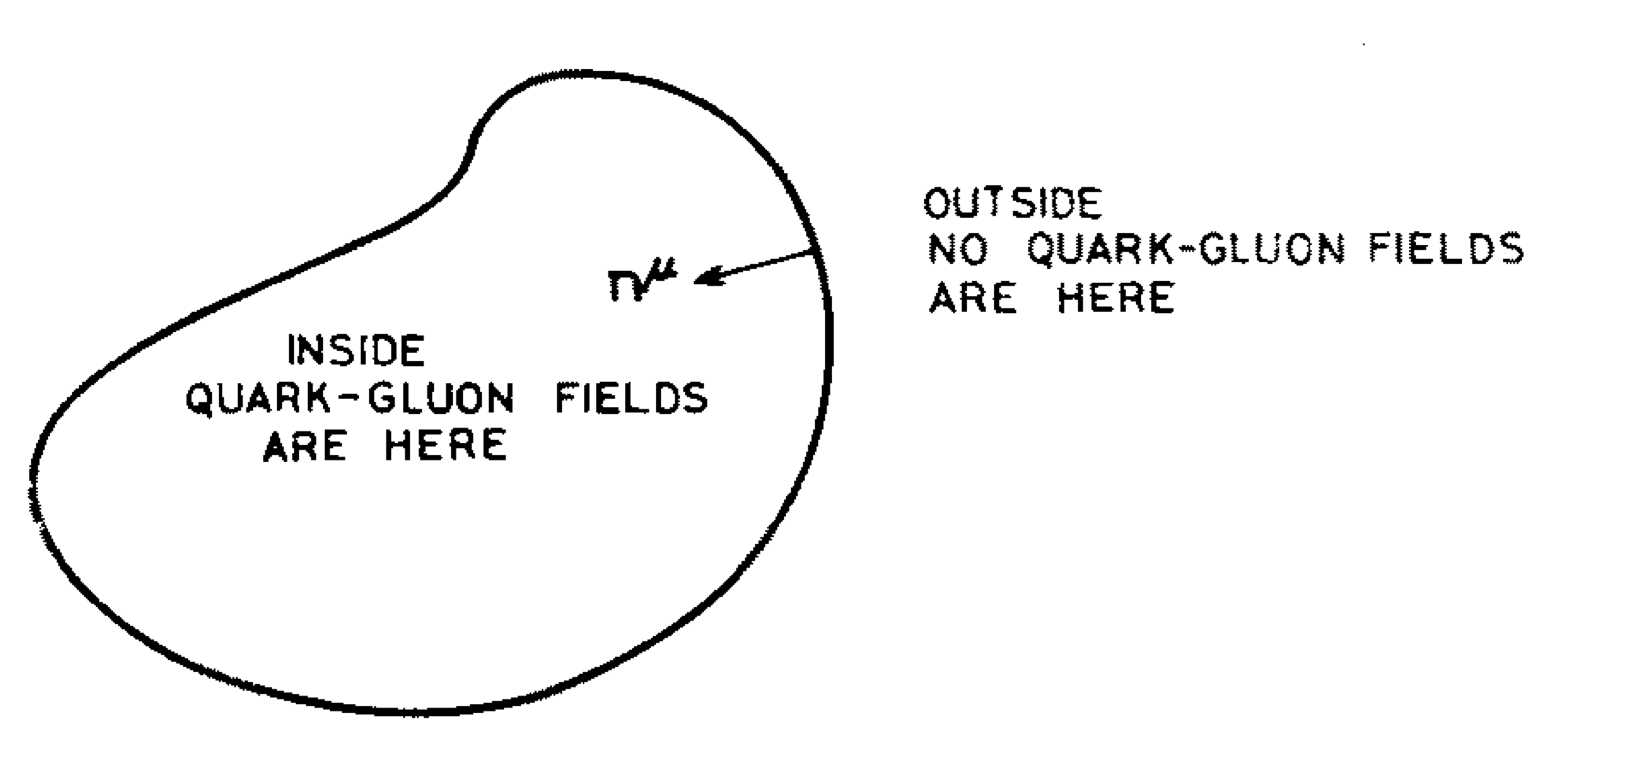
\includegraphics[width=0.4\textwidth]{./Images/Bag model BC.png}
\caption[Diagrama de bolsa con condiciones de grontera]{\emph{Dentro de la bolsa se encuentran los quarks encerrados por la presión de la bolsa.}}
\label{fig: Bolsa BC}
\end{wrapfigure}

La ecuación de Dirac (y condiciones de grontera) para el caso de una bolsa con solo quarks presentes se consigue como un extremo de la acción \eqref{eq-action} bajo variaciones en $\psi$ y $V$

\begin{equation}\label{eq-deq}
( i \slashed{\partial}_{\mu} - m) \psi= 0 \quad \mathrm{en} \, V,
\end{equation}

donde $\slashed{\partial}_{\mu} = {\partial}_{\mu} {\gamma}^{\mu}$ y con las condiciones de frontera

\begin{eqnarray}\label{eq-bc-deq}
\left.
\begin{array}{c}
i {n}^{\mu} {\gamma}_{\mu} \psi = \psi \\ 
\frac{1}{2} {n}_{\mu} {\partial}^{\mu}(\bar{\psi} \psi) = B
\end{array} 
\right\rbrace  \quad \mathrm{sobre} \, S,
\end{eqnarray}

donde ${n}_{\mu}$ es la normal interior covariante a la superficie. La primera condición de frontera \eqref{eq-bc-deq} requiere que la componente normal del vector corriente ${J}_{\mu}=\bar{\psi}{\gamma}^{\mu}{\psi}$ se elimine en la superficie. La otra condición requiere que la presión exterior del campo de quarks se equilibre con la presión de bolsa (figura \ref{fig: Bolsa BC})[referencia MIT BM].
50 Years of Quantum Chromodynamics

La solución general a las ecuaciones \eqref{eq-deq} y \eqref{eq-bc-deq} es una superposición (con coeficientes ${a}_{\alpha}$) de soluciones a la ecuación de Dirac libre:

\begin{equation}
{\psi}_{\alpha}(x,t) = \sum_{n \kappa j m} N ({\omega}_{n \kappa j}) {a}_{\alpha} (n \kappa j m) {\psi}_{n \kappa k m} (x, t).
\end{equation}

$j$ y $m$ etiquetan el modo del momento angular y su zomponente $z$. $\kappa$ es el número cuántico de Dirac\footnote{$\kappa = \pm (j + \frac{1}{2})$,},  que diferencia los dos estados de paridad opuesta para cada valor de $j$.  El índice $n$ etiqueta frecuencias que están a ser determinadas por las condiciones de frontera lineales. La  condición de fontera cuadrática (3b) restringe los modos que pueden ser excitados. Entre otras cosas, 3b permite sólo soluciones para la ecuación de Dirac.
Para $j = \frac{1}{2}$, ya sea $\kappa = - 1$,

\begin{equation}\label{eq-deq-sol-k=-1}
{\psi}_{n \, -1 \, \frac{1}{2} \, m} (x,t) = \frac{1}{\sqrt{4 \pi}} 
\left( 
\begin{array}{c}
i {j}_{0} ({\omega}_{n, \, -1} r / {R}_{0}) {U}_{m} \\
- {j}_{1} ({\omega}_{n, \, -1} r / {R}_{0}) \sigma \cdot \hat{r}{U}_{m} 
\end{array}
\right) \times {e}^{- i {\omega}_{n, \, -1} t / {R}_{0}}
\end{equation}

o ${\kappa} = 1$

\begin{equation}\label{eq-deq-sol-k=1}
{\psi}_{n \, 1 \, \frac{1}{2} \, m} (x,t) = \frac{1}{\sqrt{4 \pi}} 
\left( 
\begin{array}{c}
i{j}_{1} ({\omega}_{n, \, 1} r / {R}_{0}) \sigma \cdot \hat{r} {U}_{m} \\
{j}_{0} ({\omega}_{n, \, 1} r / {R}_{0}) {U}_{m} 
\end{array}
\right) \times {e}^{- i {\omega}_{n, \, 1} t / {R}_{0}}
\end{equation}

${U}_{m}$ es un espinos de Pauli bidimensional y ${j}_{\ell}(z)$ son las funciones de Bessel esféricas. Hemos omitido los índices $j$ sobre ${\omega}_{n \kappa}$ ya que solo $j = \frac{1}{2}$ es de interés en el presente. $N({\omega}_{n \kappa})$ es una constante de normalización escogida para conveniencia futura:

\begin{equation}
N({\omega}_{n \kappa}) \equiv \left( \frac{{\omega}_{n \kappa}^{\phantom{n \kappa} 3}}{2 {R}_{0}^{\phantom{0} 3} ({\omega}_{n \kappa} + \kappa) \sin^{2} {\omega}_{n \kappa}} \right)^{1/2}
\end{equation}

La condición de frontera lineal (3a) genera una condición eigenvalor para los modos de frecuencias ${\omega}_{n \kappa}$

$$
{j}_{0}({\omega}_{n \kappa}) = - \kappa {j}_{1} ({\omega}_{n \kappa}),
$$

o 

\begin{equation}\label{eq-condeigenval}
\tan {\omega}_{n \kappa} = \frac{{\omega}_{n \kappa}}{{\omega}_{n \kappa} + \kappa}
\end{equation}

[Por convención escogemos $n$ positiva (negativa) secuencialmente para etiquetar las raíces positivas (negativas) de la eq 7] Las primeras soluciones a \eqref{eq-condeigenval} son 

\begin{equation}\label{eq-deq-sols}
\begin{array}{ccc}
\kappa = - 1: & {\omega}_{1 \, -1} = 2.04; & {\omega}_{2 \, -1} = 5.40 \\
\kappa = + 1: & {\omega}_{1 \, 1} = 3.81; & {\omega}_{2 \, 1} = 7.00.
\end{array}
\end{equation}

La condición de frontera cuadrática requiere que $\sum_{\alpha} (\partial / \partial r) \bar{\psi}_{\alpha} (x) {\psi}_{\alpha}(x)$ sea independiente de tiempo y dirección para $r={R}_{0}$. La independencia angular requiere que $j = \frac{1}{2}$. Para obtener independencia temporal, ajustamos

\begin{equation}\label{eq-condortogon}
\sum_{\alpha} {a}_{\alpha}^{*} (n \, \kappa \, j= \frac{1}{2} \, m) {a}_{\alpha} (n' \, \kappa' \, j= \frac{1}{2} \, m') = 0,
\end{equation}

a menos que $n = n'$, $\kappa = \kappa'$ o $n = -n'$, $\kappa = -\kappa'$ en cuyos casos no hay restricción ya que los términos dependientes del tiempo se cancela. La ecuación anterior es una restricción severa sobre los modos que deben ser ocupados. Deberíamos implementar la ecuación anterior requiriendo que para cada grado de libertad interno $\alpha$ sólo un modo normal, ${a}_{\alpha}(n \, \kappa \, j = \frac{1}{2} \, m)$ es excitado. Esto automáticamente será el caso para bariones de tres quarks si son requeridos a ser singletes de color.

Una vez que \eqref{eq-condortogon} es satisfecho, los términos independientes del tiempo en \eqref{eq-deq-sol-k=1} pueden ser coleccionados,

\begin{equation}
\sum_{\alpha \, n \, \kappa \, m} {\omega}_{n \kappa} {a}_{\alpha}^{*}(n \, \kappa \, \frac{1}{2} \, m) {a}_{\alpha}(n \, \kappa \, \frac{1}{2} \, m) = 4 \pi B {R}_{0}^{4},
\end{equation}

\begin{equation}
xd
\end{equation}


\subsubsection*{Conclusiones}

\begin{enumerate}

\item El campo en la bolsa se comporta sobre el promedio como un gas relativista perfecto; que es, la traza del tensor energía momento asociado con el campo, cuando es promediado sobre tiempo y espacio, es cero:
\begin{equation}
\left\langle \int_{R} {\mathrm{d}}^{3} x ({\Theta}_{\mu}^{\mu})_{\mathrm{campo}} \right\rangle = 0
\end{equation}
\item El volumen promediado en el tiempo de una bolsa es proporcional a su energía:
\begin{equation}
E = 4B \langle V \rangle
\end{equation}
\item El estado base y estados excitados más bajos de la bolsa contienen pocos partones de momento promedio de orden ${B}^{1/4}$ encerrados en un volumen de orden ${B}^{-3/4}$. [$B$ tiene la dimensión $(\mathrm{longitud})^{-4}$ con $\hbar=c=1$]
\item En el límite termodinámico la bolsa tiene una temperatura fija, ${T}_{0}$, independiente de su energía. ${T}_{0}$ es de orden ${B}^{-1/4}$. Esto es equivalente a las siguientes declaraciones
\begin{itemize}
\item La energía cinética promedio de los partones es de orden ${T}_{0}$ independiente de la energía de bolsa $E$ proporcionado el último es más grande que ${T}_{0}$: ${E} \gg {T}_{0}$.
\item La densidad de nivel asintótico ${\zeta(E)}$ del sistema es una función exponencial de $E$:
\[
\zeta \sim {e}^{E/{T}_{0}}
\]
\item El número, $N$, de partones más antipartones presente en el hadrón es proporcional a su energía:
\[
N \propto E/{T}_{0}
\]
\end{itemize}
\item Si la dinámica clásica es tal que hay un máximo momento angular del hadrón en una energía total dada $E$, ese máximo debe ser 
\[
{J}_{\mathrm{m\acute{a}x}} = \kappa {B}^{-1/3} {E}^{4 / 3},
\]
donde ${\kappa}$ es una constante adimensional determinada por la dinámica detallada. Si el límite clásico $({\hbar} \rightarrow 0)$ existe, las correcciones cuánticas a esta fórmula se reducirían por potencias de $E$. Si no hay trayectoria clásica a seguir, un argumento plausible sugiere que la trayectoría guía podría ser (para un gran $E$)
\[
{J}_{\mathrm{m\acute{a}x}} = {\kappa}' {B}^{-1/2} {E}^{2} \quad ({\hbar = 1}).
\]
\item El momento angular más probable para una $E$ grande está dada por 
\[
\bar{J} \propto ({B}^{-1/4} E)^{5/6}
\]
\end{enumerate}

%\subsection{Refinamientos que corrigen el movimiento del centro de masa}
%
%Una de las características incómodas de la aproximación de cavidad que es compartida por modelos de caparazón en general es que el centro de masa (c.m.) del estado de muchos cuerpos es en movimiento, y la energía cinética de movimiento es inevitablemente incluida en la energía orbital total. Esta contribución debería ser removida de la energía de bolsa para obtener la masa. En el modelo de caparazón nuclear es posible proyectar estados no relativistico de  momento definito de centro de masa. El Hamiltoniano cuántico invariante traslacionalmente subyacente es conocido, y la energía corregida del estado puede ser determinada (53). En la aproximación de cavidad, sin embargo, el Hamiltoniano cuántico es definido sólo con respecto a una cavidad particular y no es traslacionalmente invariante. No existe proyección sobre eigenestados de momento. 
%
%No hay procedimientos unívoco para corregir el movimiento de centro de masa. Sin embargo, varias aproximaciones han sido intentadas. En el método de Donoghue \& Johnson, el estado de bolsa con números cuánticos de nucleones no es precisamente identificado con el núcleon; en vez de eso, es considerado más generalmente como un paquete de ondas de estados de momentos de nucleones con un momento generalizado promedio $\langle \vb{p} \rangle = 0$ pero $\langle {p}^{2} \rangle \neq 0$. La energía de bolsa no es entonces precisamente la masa de la partícula, sino
%
%\begin{equation}
%{E}_{\mathrm{bolsa}} = \langle H \rangle =  \langle \sqrt{{p}^{2} + {m}^{2}} \rangle.
%\end{equation}
%
%Para la mayoría de estados (esos con $m \gg 1 / R$), la expansión no relativistica es posible: ${E}_{\mathrm{bolsa}}$. La corrección podría ser estimada en varias formas. 
%
%\section{Other models}
%
%\begin{equation}
%6
%\end{equation}

%
%\section{Una variedad de estados de bolsa}
%
%\subsection{Cuerdas}
%
%Las partículas de estado base han sido asumidas que corresponden a una bolsa esférica.
%

%\section{Interacciones}
%
%\subsection{Interacciones electrodébiles}
%
%El modelo de bolsa ha sido extensivamente usada como una herramienta en el estudio de las propiedades débiles y electromagnéticas de hadrones. No somos capaces de describir todas las aplicaciones, pero en vez de eso concentrar sobre las propiedades estáticas de los bariones (25, 34, 43, 86). Primero describimos los resultados no corregidos de (43). Cuatro tipos de corrección han sido estudiadas: 
%
%\begin{enumerate}
%\item retroceso del centro de masa
%\item intercambio de gluones
%\end{enumerate}
%
%Para el radio de carga del protón  DeGrand et al(43) obtiene
%
%$$
%\langle {r}^{2} \rangle_{\mathrm{EM}} = 0.55 {R}^{2} = (0.73 \; \mathrm{\unit{\femto\meter}})^{2}
%$$
%
%$$
%[\mathrm{experimento:} \quad \langle {r}^{2} \rangle_{\mathrm{EM}} = (0.90 \; \mathrm{\unit{\femto\meter}})^{2}]
%$$
%
%para quarks sin masa. [Para los valores de esta y otras cantidades en masa de quark no cero, ver (34, 86).] Este resultado es significante debido a que significa que el modelo de bolsa predice muy correctamente cercano el tamaño del protón. Tal conexión entre la masa y radio es no trivial. De hecho, usando el radio apropiado es a menudo más importante que tener la masa correcta, porque es el radio el que determina la escala de la mayoría de los elementos de matriz.
%
%El momento magnético de un estado puede ser calculado por el elemento de matriz del primer momento de corriente electromagnética
%
%\begin{equation}
%\langle \vb{\mu} \rangle = \langle \int \mathrm{d}^{3} x \frac{1}{2} \vb{x} \times \vb{J} (x) \rangle.
%\end{equation}
%
%Esta definición del momento incluye las contribuciones debida a ambas el flujo de carga y el espín del quark. En el límite no relativistíco, se reduce al usual
%
%\begin{equation}
%\vb{\mu} = \sum_{i} \frac{{Q}_{i} {\vb{\sigma}}_{i}}{2 {m}_{i}},
%\end{equation}
%
%mientras que para quarks sin masa en el protón, es
%
%\begin{equation}
%\vert {\mu}_{\mathrm{p}} \vert = 0.20 R e.
%\end{equation}
%
%Los parámetros de DeGrand et al llevan a una muy pequeña razón giromagnética (${g}_{\mathrm{p}} = 2{m}_{\mathrm{p}} {\mu}_{\mathrm{p}} / e = 1.9$)